%% =====================================================================
%% CO-PRIOR — research proposal (VEGA house style, ACM acmart/sigplan)
%% Compile: pdflatex main && bibtex main && pdflatex main && pdflatex main
%% Requires acmart.cls + ACM-Reference-Format.bst beside this file.
%% =====================================================================
\documentclass[sigplan,nonacm,screen]{acmart}

\AtBeginDocument{\providecommand\BibTeX{{Bib\TeX}}}
\settopmatter{printacmref=false}
\renewcommand\footnotetextcopyrightpermission[1]{}

%% ---------- figures, algorithms, boxes, colour ----------
\usepackage{tikz}
\usetikzlibrary{arrows.meta,positioning,shapes.geometric,calc,fit,backgrounds}
\usepackage[most]{tcolorbox}
\usepackage{amsmath}
\usepackage{algorithm}
\usepackage{algpseudocode}

%% ---------- diagram style: strictly BLACK-ON-WHITE ----------
\tikzset{
  box/.style={draw=black, fill=white, rectangle, rounded corners=1.5pt, align=center,
              inner sep=4pt, minimum height=8mm, font=\footnotesize},
  bigbox/.style={box, line width=1pt, minimum width=26mm, minimum height=13mm},
  small/.style={box, font=\scriptsize, inner sep=3pt},
  dec/.style={draw=black, fill=white, diamond, aspect=2.2, align=center,
              inner sep=1pt, font=\scriptsize, minimum height=9mm},
  fl/.style={-{Stealth[length=2mm]}, thick, black},
  flthin/.style={-{Stealth[length=1.6mm]}, thin, black},
  flthick/.style={-{Stealth[length=2.8mm]}, line width=1.3pt, black},
  lbl/.style={font=\scriptsize, midway, fill=white, inner sep=1pt},
}

%% ---------- coloured callout boxes ----------
\tcbset{vegabox/.style={enhanced, breakable, boxrule=0.5pt, arc=2pt,
  left=5pt,right=5pt,top=3pt,bottom=3pt,
  fonttitle=\bfseries\small, coltitle=white,
  colupper=black, colback=white}}
\newtcolorbox{defbox}[1][Definition]{vegabox, colback=blue!4,
  colframe=blue!55!black, colbacktitle=blue!55!black, title=#1}
\newtcolorbox{exbox}[1][Everyday example]{vegabox, colback=orange!7,
  colframe=orange!72!black, colbacktitle=orange!72!black, title=#1}
\newtcolorbox{keybox}[1][Key insight]{vegabox, colback=green!6,
  colframe=green!48!black, colbacktitle=green!48!black, title=#1}
\newtcolorbox{gapbox}[1][Research gap]{vegabox, colback=red!4,
  colframe=red!62!black, colbacktitle=red!62!black, title=#1}

\setlength{\parskip}{2.5pt plus 1pt minus 1pt}

\begin{document}

\title{CO-PRIOR: Composing Disjoint-Cohort Experts for Flexible Cervical Cancer Screening}
\subtitle{Prior-stripped opinion pooling, and the price of an assumption you cannot avoid paying}

\author{First Author}
\affiliation{%
  \institution{Department of Computer Science, Your University}
  \city{City}\country{Country}}
\email{rsgidristee@gmail.com}
\renewcommand{\shortauthors}{Author et al.}

\begin{abstract}
Cervical cancer is almost entirely preventable, yet the two cheapest screening signals---a Pap-smear cell image and a patient risk questionnaire---are only ever published as \emph{separate} datasets with no shared patients and different label spaces. A flexible screener that accepts either or both is therefore blocked at the first step: every missing-modality method we verified needs a \emph{paired anchor} somewhere (a complete-modality teacher~\cite{wei2023mmanet}, a shared encoder~\cite{wang2023shaspec}, learned priors~\cite{ma2021smil}, or paired pretraining). Two failure modes make the naive fix worse than useless. \emph{First}, the tabular arm's published accuracy is an artefact: leakage-safe nested cross-validation puts UCI biopsy prediction at $\mathrm{AUROC}=0.656$ (95\% CI $[0.584,0.720]$), against a literature reporting $0.98$--$1.00$~\cite{roy2025interpretable}; predicting \texttt{Dx:Cancer} from its sibling \texttt{Dx} columns alone scores $0.998$. \emph{Second}, naive late fusion can \emph{lose}: an image$+$tabular late-fusion system scored $92\%$ against $96\%$ for its tabular expert alone~\cite{kelebet2025multimodal}. We propose \textbf{CO-PRIOR}, whose single claim is the \emph{two-prior composition operator}: because each expert's posterior is contaminated by its own cohort's prevalence, we \emph{strip} each prior out before pooling and apply one declared deployment prior afterwards. \emph{Honest novelty note:} the pooling rule itself is \textbf{borrowed}---it is ProbEn~\cite{chen2022proben} and, one level up, a weighted opinion pool~\cite{genest1986combining}; calibration across modality subsets is \textbf{borrowed} from AECF~\cite{chlon2025aecf}; only the prior-stripping precondition is \textbf{ours}. Crucially it is validatable \emph{per expert} on public data. We evaluate on SIPaKMeD~\cite{plissiti2018sipakmed}, Herlev, HiCervix~\cite{cai2024hicervix} and UCI~\cite{fernandes2017transfer}, against \texttt{max(image-only, tabular-only)}, with a pre-registered falsifier.
\end{abstract}

\begin{CCSXML}
<ccs2012>
<concept><concept_id>10010147.10010257</concept_id>
<concept_desc>Computing methodologies~Machine learning</concept_desc>
<concept_significance>500</concept_significance></concept>
<concept><concept_id>10010405.10010481</concept_id>
<concept_desc>Applied computing~Health informatics</concept_desc>
<concept_significance>300</concept_significance></concept>
</ccs2012>
\end{CCSXML}
\ccsdesc[500]{Computing methodologies~Machine learning}
\ccsdesc[300]{Applied computing~Health informatics}

\keywords{decision-level fusion, missing modality, calibration, prior shift, conformal prediction, cervical cancer screening, data leakage}

\maketitle

%% =====================================================================
\section{Introduction}

\subsection{Background for the non-specialist}

Cervical cancer is caused by persistent infection with high-risk human papillomavirus (HPV). It progresses slowly through detectable pre-cancerous stages, which is why screening works so well: catch the lesion early and the disease is preventable. The bottleneck is not biology---it is access to the expert who reads the slide.

\begin{defbox}[The two signals this proposal combines]
\textbf{Pap-smear cytology.} Cells are scraped from the cervix, stained, and examined under a microscope. A trained cytopathologist looks for abnormal cell shapes. This is a \emph{finding}: it looks at the disease itself.\\[3pt]
\textbf{Risk questionnaire.} A form recording age, number of pregnancies, smoking, contraceptive use, and sexually-transmitted-infection history. This is a \emph{pre-test risk}: it estimates how likely a problem is \emph{before} anyone looks.
\end{defbox}

\begin{exbox}[Two very different colleagues]
Think of the image model as a \emph{pathologist} who looks down the microscope at your actual cells, and the questionnaire model as a \emph{receptionist} who glances at your intake form. The pathologist sees the disease; the receptionist only knows that people with your profile tend to be higher risk. You would happily let the receptionist say ``bump this patient up the queue''---but you would never let them overrule the pathologist. Almost everything in this proposal follows from taking that asymmetry seriously.
\end{exbox}

The naive engineering picture is: train a model on each signal, average their outputs, ship a system that works with either. Every step of that picture fails in a way the literature has documented but not solved, and the rest of this section says exactly how.

\subsection{The problems}

\paragraph{Problem 1: the questionnaire model's reported accuracy is an artefact.}
The near-universal substrate for cervical risk modelling is the UCI \emph{Cervical Cancer (Risk Factors)} dataset~\cite{fernandes2017transfer}: 858 patients, 36 attributes, four binary screening targets. Published models report $0.98$--$1.00$ AUC on it---for example a stacking ensemble reporting $0.98$ accuracy and $0.995$ AUC using SMOTE~\cite{chawla2002smote} and, by the authors' own statement, no external validation~\cite{roy2025interpretable}.

\begin{exbox}[Why that number is not real]
Two mistakes produce it. \emph{(1) Studying the answer sheet.} The dataset ships \texttt{Dx:Cancer}, \texttt{Dx:CIN}, \texttt{Dx:HPV} and \texttt{Dx}---records of \emph{past diagnoses}. Predicting one from the others is not diagnosis, it is copying. \emph{(2) Photocopying the exam before splitting it.} SMOTE invents synthetic minority patients; if you do that \emph{before} the train/test split, synthetic copies of a test patient end up in training. The model has seen the test.
\end{exbox}

This is measured, not hypothetical. Under leakage-safe nested cross-validation---\texttt{Dx:*} dropped, resampling confined inside folds---we obtain $\mathrm{AUROC}=0.656$ (95\% CI $[0.584, 0.720]$) for the biopsy target, and a tuned bake-off over eight model families does not exceed $\approx0.65$. Predicting \texttt{Dx:Cancer} from its sibling \texttt{Dx} columns scores $0.998$; from legitimate features only, $0.592$. No single feature exceeds a univariate AUROC of $0.572$. The dataset's own creators, using stratified $10$-fold with nested inner cross-validation and \emph{no} oversampling, are the honest anchor here~\cite{fernandes2018supervised}.

\paragraph{Problem 2: the data is unpaired, and that is structural.}
No public dataset pairs a cervical image with a risk questionnaire \emph{for the same patient}. SIPaKMeD ($4{,}049$ cells from $966$ cluster images)~\cite{plissiti2018sipakmed}, Herlev, and HiCervix ($40{,}229$ cells from $4{,}496$ slides)~\cite{cai2024hicervix} carry \emph{no} patient metadata at all. The barrier is consent and de-identification, not effort: the datasets were collected anonymously, so age and history cannot be recovered by re-annotation.

\paragraph{Problem 3: fusion can make things worse, and nobody checks.}
An image$+$tabular late-fusion system for cervical risk scored $92\%$---while its own tabular expert alone scored $96\%$~\cite{kelebet2025multimodal}. Meanwhile calibration, the property that decides whether a screening score can be trusted, is absent: across the missing-modality and cervical-fusion literatures we verified, calibration is not reported at all.

\subsection{The gap, and the idea in one picture}

Two mature literatures sit either side of our problem and never meet. One \emph{corrects a single classifier's prior} when it is deployed into a population with a different prevalence~\cite{saerens2002adjusting,godau2023deployment,alexandari2020maximum}. The other \emph{combines several classifiers}---but always assuming they share one prior~\cite{kittler1998combining,genest1986combining,chen2022proben}.

\begin{gapbox}[G3 --- the two-prior gap]
Nobody performs prior-\emph{stripping} as a \textbf{precondition of pooling}. Yet two experts trained on two cohorts necessarily carry \emph{two different} baked-in prevalences: our image expert sees $\approx40\%$ abnormal cells (a labelling choice), the questionnaire expert $\approx6.4\%$ biopsy-positive patients (a clinic's case mix). Neither is a deployment prevalence. Pooling them raw counts an accident of dataset construction as if it were evidence.
\end{gapbox}

\begin{figure}[t]\centering
\resizebox{0.95\columnwidth}{!}{%
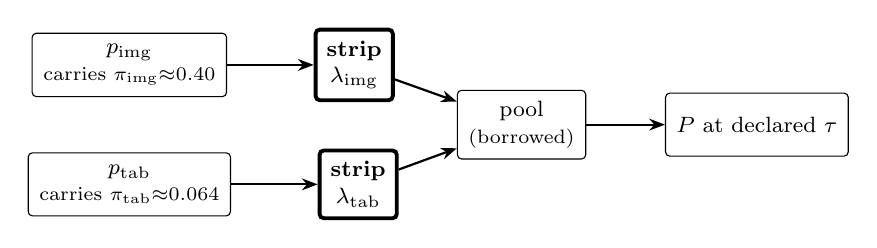
\begin{tikzpicture}[node distance=5mm and 9mm, newm/.style={box, line width=1.4pt}]
  \node[box] (pi) {$p_{\mathrm{img}}$\\\scriptsize carries $\pi_{\mathrm{img}}{\approx}0.40$};
  \node[box, below=7mm of pi] (pt) {$p_{\mathrm{tab}}$\\\scriptsize carries $\pi_{\mathrm{tab}}{\approx}0.064$};
  \node[newm, right=11mm of pi] (si) {\textbf{strip}\\$\lambda_{\mathrm{img}}$};
  \node[newm, right=11mm of pt] (st) {\textbf{strip}\\$\lambda_{\mathrm{tab}}$};
  \node[box] (pool) at ($(si)!0.5!(st)+(2.1,0)$) {pool\\\scriptsize (borrowed)};
  \node[box, right=10mm of pool] (out) {$P$ at declared $\tau$};
  \draw[fl](pi)--(si); \draw[fl](pt)--(st);
  \draw[fl](si)--(pool); \draw[fl](st)--(pool); \draw[fl](pool)--(out);
\end{tikzpicture}}
\caption{\textbf{The idea.} Each expert's posterior is contaminated by its own cohort's prevalence. We divide that prior out (thick boxes = our contribution), pool the resulting prior-free evidence with a \emph{borrowed} rule, then apply one \emph{declared} deployment prior $\tau$ once.}
\Description{Two posteriors, each carrying its own training prevalence, pass through prior-stripping blocks into a pooling block and out to a probability at a declared prevalence.}
\label{fig:idea}
\end{figure}

\subsection{Contributions}
\begin{itemize}
  \item \textbf{The two-prior composition operator (core).} Prior-stripping as a precondition of pooling experts trained on disjoint cohorts---the one operation the prior-correction and classifier-combination literatures each leave to the other. Validatable \emph{per expert}, without any paired cohort.
  \item \textbf{A leakage-audited honest baseline for UCI (core).} No prior work satisfies all three of \{\texttt{Dx:*} dropped, resampling confined inside folds, calibration reported\}. We supply it: $0.656$ $[0.584,0.720]$, with a two-factor decomposition of where $0.98$--$1.00$ comes from.
  \item \textbf{The price of a forced assumption.} At zero cohort overlap the cross-modal dependence is \emph{non-identified}, so conditional independence is forced, not chosen. We transport a quantified, \emph{directional} penalty from biostatistics (over-estimation of risk up to $56\%$~\cite{grill2017comparison}) into a pre-registered prediction about our own output.
  \item \textbf{An honest impossibility result.} We show what a disjoint-cohort screener can and cannot be validated to do---and report the both-modality path as unvalidatable rather than asserting a number.
\end{itemize}

%% =====================================================================
\section{Related Work}

\subsection{Image-only cervical AI}
One line of work classifies single cells with progressively stronger backbones---CNNs, then vision transformers---on SIPaKMeD~\cite{plissiti2018sipakmed} and Herlev, reporting accuracies above $95\%$. It works because the benchmarks are curated, balanced, pre-segmented single cells. A second line scales to whole slides with cervical foundation models: Smart-CCS pretrains on $127{,}471$ slides across $48$ centres and reports internal AUC $0.965$ and external $0.950$~\cite{zhang2025smartccs}. The shared limitation is transfer: our own SIPaKMeD-trained expert scores $0.998$ in-distribution but $0.73$ on Herlev, $0.59$ on HiCervix and $0.53$ on APACC. Worse, SIPaKMeD and Herlev publish \emph{no patient identifiers}, so a patient-wise split is impossible \emph{in principle}---cells cropped from one slide can land on both sides of a random split.

\begin{gapbox}[Recurring limitation]
These systems classify images ever more accurately on the benchmark they were trained on; \emph{none} reports whether its confidence is trustworthy, and none degrades gracefully when the image is unavailable.
\end{gapbox}

\subsection{Tabular cervical risk models}
A second family fits classical learners---random forests, boosting, stacking ensembles---to the UCI questionnaire and reports $0.98$--$1.00$ AUC~\cite{roy2025interpretable}. The pattern is consistent: oversample with SMOTE~\cite{chawla2002smote}, keep the \texttt{Dx:*} columns, evaluate on a single Venezuelan cohort, report accuracy. Gradient-boosted trees are the right model family for tables of this size~\cite{grinsztajn2022why}; the problem is not the learner but the protocol. The honest anchor exists and is by the dataset's own creators, who use nested cross-validation without oversampling~\cite{fernandes2018supervised}.

\begin{gapbox}[Recurring limitation]
No paper satisfies all three of: \texttt{Dx:*} excluded, resampling confined inside folds, calibration reported. The field's headline numbers measure leakage, not risk.
\end{gapbox}

\subsection{Missing-modality and multimodal fusion}
A large literature makes multimodal models survive an absent input. HeMIS-style averaging, SMIL's learned modality priors~\cite{ma2021smil}, ShaSpec's shared/specific decomposition~\cite{wang2023shaspec}, MMANet's complete-modality teacher~\cite{wei2023mmanet}, and prompt-conditioned transformers~\cite{lee2023multimodal} all work---and all need the same thing. As their own survey confirms~\cite{wu2024survey}, the mechanism is learned from samples where the modalities are \emph{co-observed}. Even the work that explicitly rejects jointly-pretrained encoders still ``requires modality-complete data during training''~\cite{kim2024missing}. Closest to us in spirit: AECF enforces monotone confidence across \emph{all} modality subsets and measures per-subset ECE~\cite{chlon2025aecf}; Gu et al.\ fuse image and tabular data with modality dropout~\cite{gu2025modality}. Both train on \emph{paired} data with \emph{simulated} masking.

\begin{gapbox}[Recurring limitation]
Every method assumes a paired anchor exists somewhere. At \emph{zero} overlap---two cohorts, no shared patient, different label spaces---the anchor cannot be built, and imputation has nothing to impute from.
\end{gapbox}

\subsection{Composition, calibration, and abstention}
The theory we actually need is older and lives outside cervical AI. Kittler et al.\ derive the sum and product rules and show the sum rule is more robust to individual estimation error~\cite{kittler1998combining}; Genest and Zidek characterise opinion pooling generally~\cite{genest1986combining}; ProbEn applies Bayes' rule with conditional independence and marginalises over absent modalities~\cite{chen2022proben}. On the calibration side, temperature scaling is standard~\cite{guo2017calibration}, and prior correction has a canonical EM procedure~\cite{saerens2002adjusting} with a modern successor that warns the procedure presupposes calibration---``which is not true of modern neural networks''~\cite{alexandari2020maximum}. Uncertainty can be made explicit with evidential heads~\cite{sensoy2018evidential,han2021trusted,han2023trusted}, though the resulting mass is a \emph{relative} signal, and quality-aware fusion needs the per-view scales to be comparable~\cite{zhang2023provable}. Conformal prediction supplies distribution-free guarantees~\cite{angelopoulos2021gentle}, but they are \emph{marginal}, and under label shift they degrade unless unlabeled target data is available~\cite{podkopaev2021distribution}.

\begin{gapbox}[Recurring limitation]
One literature retargets \emph{one} classifier to \emph{one} population; the other combines \emph{several} classifiers under a \emph{common} prior. Neither strips priors as a precondition of pooling---which is exactly what two disjoint cohorts force you to do.
\end{gapbox}

%% =====================================================================
\section{Research Gaps}

\paragraph{G1 --- Every missing-modality method needs a paired anchor.}
\begin{itemize}
  \item \emph{Evidence.} Complete-modality teacher~\cite{wei2023mmanet}; shared encoder trained on co-observed modalities~\cite{wang2023shaspec}; priors learned where the modality is observed~\cite{ma2021smil}; frozen paired backbone~\cite{lee2023multimodal}; ``requires modality-complete data during training''~\cite{kim2024missing}; confirmed by the field survey~\cite{wu2024survey}.
  \item \emph{Why open.} The dependency is architectural, not incidental. At zero overlap there is nothing to anchor to.
  \item \emph{This proposal's answer.} M5: an absent expert contributes the additive identity---no imputation, no anchor.
\end{itemize}

\paragraph{G2 --- Calibration is unreported, and nobody asks whether confidence should drop when a modality is missing.}
\begin{itemize}
  \item \emph{Evidence.} Not reported across the missing-modality and cervical-fusion work we verified; the counter-example is AECF, on paired non-medical data~\cite{chlon2025aecf}.
  \item \emph{Why open.} A screening score that cannot say ``I am less sure now'' is unsafe in exactly the case flexible inference creates.
  \item \emph{This proposal's answer.} M3 + H-D: monotone confidence in the evidence set, measured.
\end{itemize}

\paragraph{G3 --- No method composes two experts carrying two different priors.}
\begin{itemize}
  \item \emph{Evidence.} Prior correction is one-classifier-one-population~\cite{saerens2002adjusting,godau2023deployment,alexandari2020maximum}; combination assumes a common prior~\cite{kittler1998combining,genest1986combining,chen2022proben}.
  \item \emph{Why open.} It is a hole in the theory, and it is unavoidable once cohorts differ.
  \item \emph{This proposal's answer.} \textbf{M4 --- the operator we claim.}
\end{itemize}

\paragraph{G4 --- The only available fusion route is the one that miscalibrates most.}
\begin{itemize}
  \item \emph{Evidence.} Independence over-estimates risk by up to $56\%$~\cite{grill2017comparison}; naive late fusion lost to its own tabular expert, $92\%$ vs $96\%$~\cite{kelebet2025multimodal}.
  \item \emph{Why open.} At zero overlap the dependence is non-identified: the assumption is forced.
  \item \emph{This proposal's answer.} M7: report an envelope over the unknown dependence, and pre-register the predicted direction of the error.
\end{itemize}

\paragraph{G5 --- Both arms sit on leakage-inflated benchmarks.}
\begin{itemize}
  \item \emph{Evidence.} $0.98$--$1.00$ published~\cite{roy2025interpretable} vs $0.656$ leakage-safe (ours) and the creators' nested-CV anchor~\cite{fernandes2018supervised}; no patient IDs in SIPaKMeD/Herlev.
  \item \emph{Why open.} Nobody has run the audit on this dataset.
  \item \emph{This proposal's answer.} RQ1 + ablations A3/A4.
\end{itemize}

\begin{table}[t]
\caption{Gaps mapped to the module that answers them and the question that tests them.}
\label{tab:gapmap}
\footnotesize
\setlength{\tabcolsep}{4pt}
\begin{tabular}{@{}llp{2.1cm}@{}}
\toprule
\textbf{Gap} & \textbf{Module} & \textbf{RQ} \\
\midrule
G1 paired anchor required & M5 router & RQ4 \\
G2 calibration unreported & M3, M8 & RQ4 \\
\textbf{G3 two priors} & \textbf{M4 (ours)} & \textbf{RQ2} \\
G4 forced independence & M7 envelope & RQ3 \\
G5 leakage & M2 protocol & RQ1 \\
\bottomrule
\end{tabular}
\end{table}

%% =====================================================================
\section{Research Questions and Hypotheses}

\begin{description}
  \item[RQ1 (honest baseline).] What is the leakage-free ceiling of the UCI questionnaire for biopsy, and how much of the published $0.98$--$1.00$ is leakage?
  $H_0$: the leakage-safe AUROC is statistically indistinguishable from the published figure. $H_1$: it is far lower, and the difference is accounted for by target leakage plus pre-split resampling.
  \item[RQ2 (the operator).] Does stripping each expert's own prior \emph{before} pooling produce better-calibrated composed posteriors than pooling raw posteriors?
  $H_0$: $\Delta\mathrm{ECE}=0$. $H_1$: $\Delta\mathrm{ECE}<0$ (stripping helps), growing with the gap between the two priors.
  \item[RQ3 (the price).] What is the magnitude and direction of the miscalibration caused by the forced independence assumption, and over what dependence range does composition beat the better single expert?
  $H_0$: composition is unbiased and always helps. $H_1$: it is \emph{over-confident} in a predictable direction, and the gain is $\le 0$ for realistic dependence.
  \item[RQ4 (confidence under absence).] Is confidence monotone in the available evidence set, and does per-path calibration survive prevalence shift?
  $H_0$: confidence is unchanged when a modality is removed. $H_1$: confidence decreases, and no subset is more confident than a superset containing it.
\end{description}

\paragraph{Pre-registered hypotheses.}
\begin{description}
  \item[H-A.] Leakage-safe UCI biopsy AUROC $\le 0.75$ (upper CI bound). \emph{Metric:} AUROC + BCa CI.
  \item[H-B.] Honest AUROC plus the two leakage increments reconstructs the published figure to within $0.02$, leaving no residual signal.
  \item[H-C.] $\Delta\mathrm{ECE}$(stripped $-$ raw) $<0$, and its magnitude grows with $|\mathrm{logit}\,\pi_{\mathrm{img}}-\mathrm{logit}\,\pi_{\mathrm{tab}}|$.
  \item[H-D.] Mean confidence is monotone: both $\ge$ single $\ge$ prior-only, with zero superset violations.
  \item[H-E \emph{(falsifier)}.] \emph{On the realistic operating point, composition does \emph{not} beat} \texttt{max(image-only, tabular-only)} \emph{on AUROC beyond noise}---stated up front, because both experts are HPV-driven and therefore positively dependent, which is precisely where pooling stops paying. If H-E holds, we report the negative result; the precedent for it being real is~\cite{kelebet2025multimodal}.
\end{description}

%% =====================================================================
\section{Proposed Methodology}

\subsection{Design philosophy and honest positioning}

CO-PRIOR is deliberately small. Everything that can be borrowed \emph{is} borrowed, so that the contribution is a single, testable operation rather than a system. The two experts are frozen; every component after them is closed-form and costs microseconds; and every component is fitted \emph{on one cohort at a time}, because that is the only regime in which anything here can be validated.

\begin{keybox}[What is NOT novel]
We do \emph{not} claim the fusion rule: applying Bayes' rule under conditional independence and marginalising over absent modalities is ProbEn~\cite{chen2022proben}, and one level up it is a weighted opinion pool, a literature characterised forty years ago~\cite{genest1986combining}. We do \emph{not} claim calibrated confidence across modality subsets: AECF claims \emph{and measures} it~\cite{chlon2025aecf}. We do \emph{not} claim modality dropout for image$+$tabular: that is Gu et al.~\cite{gu2025modality}. We do \emph{not} claim prior correction: that is Saerens et al.~\cite{saerens2002adjusting}, superseded by~\cite{alexandari2020maximum}. \textbf{Our contribution is the precondition}: stripping each expert's own prior \emph{before} the pool, which neither literature does.
\end{keybox}

\begin{table}[t]
\caption{Borrowed / modified / new. The novelty is one row.}
\label{tab:novelty}
\footnotesize
\setlength{\tabcolsep}{4pt}
\begin{tabular}{@{}llp{2.3cm}@{}}
\toprule
\textbf{Component} & \textbf{Status} & \textbf{Closest prior} \\
\midrule
M1 image expert & borrowed & \cite{tan2019efficientnet,plissiti2018sipakmed} \\
M2 tabular expert & borrowed & \cite{grinsztajn2022why} \\
M2 leakage protocol & modified & \cite{fernandes2018supervised} \\
M3 calibration & borrowed & \cite{guo2017calibration,alexandari2020maximum} \\
\textbf{M4 prior-stripping} & \textbf{NEW} & \emph{none found} \\
M5 availability router & borrowed & \cite{chen2022proben} \\
M6 pooling rule & borrowed & \cite{kittler1998combining,genest1986combining} \\
M7 dependence envelope & modified & \cite{grill2017comparison} \\
M8 conformal abstention & borrowed & \cite{angelopoulos2021gentle} \\
M9 modality attribution & modified & --- \\
\bottomrule
\end{tabular}
\end{table}

\subsection{Why not Bethesda?}
\label{sec:bethesda}

A reader who knows cytology will object immediately: there \emph{is} a standard shared language for cervical results, so why invent a binary axis?

\begin{defbox}[The Bethesda System (TBS)]
TBS is the international standard for reporting cervical cytology~\cite{nayar2015pap}. It grades a slide on an ordered scale---\textsc{nilm} (negative), \textsc{asc-us} (atypical squamous cells of undetermined significance), \textsc{lsil} (low-grade lesion), \textsc{asc-h}, \textsc{hsil} (high-grade lesion), up to carcinoma---plus glandular categories (\textsc{agc}). It is the language in which a real Pap result is reported and acted upon.
\end{defbox}

TBS is the obvious candidate bridge, and we considered it seriously. It fails here for three reasons, and the third is the interesting one.

\begin{itemize}
  \item \textbf{SIPaKMeD cannot populate TBS.} Its five classes are cell \emph{types}, not diagnoses: \emph{Parabasal}, \emph{Metaplastic} and \emph{Superficial-Intermediate} are normal cell categories, and \emph{Koilocytotic} names an HPV cytopathic effect rather than a grade. The mapping to TBS is one-to-many at the fine level. Decisively, the dataset contains no high-grade category at all: a model trained on it \emph{cannot express \textsc{hsil}}---the grade that carries the clinical risk. A TBS axis with no \textsc{hsil} is not a TBS axis.
  \item \textbf{The UCI target that would align with TBS carries no signal.} \texttt{Citology} is the natural counterpart of a Pap report. Under our leakage-safe protocol it scores $\mathrm{AUROC}=0.488$ (95\% CI $[0.407,0.575]$)---at or below chance. Aligning the constructs via TBS routes the system to the one target with nothing in it.
  \item \textbf{TBS does not touch the unit mismatch.} A Bethesda report describes a \emph{slide}; SIPaKMeD describes a \emph{cell}. Relabelling the axis does not tell you how to turn many cell verdicts into one patient verdict, and no public data can calibrate that aggregation because no patient identifiers exist.
\end{itemize}

\begin{keybox}[What Bethesda actually teaches us]
TBS would make the shared axis more clinically \emph{legible} without making the two constructs \emph{commensurable}---it relabels the problem rather than solving it. That is itself evidence for this proposal's central claim: the image label and the biopsy label are not two noisy readings of one variable. \emph{Where a dataset natively provides TBS we use it}: HiCervix ships a three-level Bethesda hierarchy over $40{,}229$ cells~\cite{cai2024hicervix}, and we use it for \emph{external validation}---collapsing \textsc{nilm} to negative and \textsc{lsil}/\textsc{hsil}/\textsc{asc-us}/\textsc{asc-h}/carcinoma to positive, while \emph{excluding} glandular categories the image expert provably cannot see.
\end{keybox}

\subsection{The construct and unit mismatch}

\begin{figure}[t]\centering
\resizebox{0.86\columnwidth}{!}{%
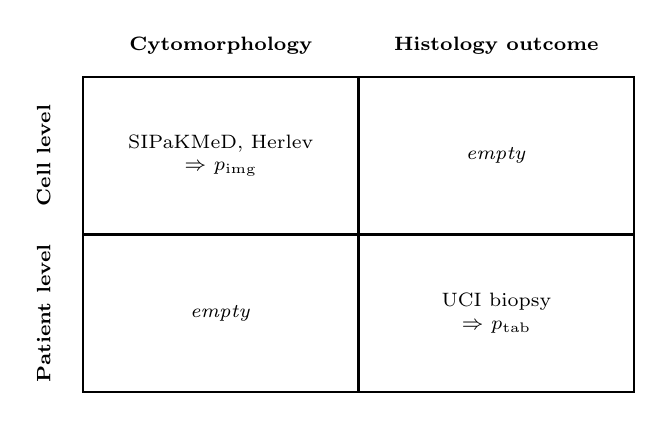
\begin{tikzpicture}
  \draw[thick] (0,0) rectangle (7,4);
  \draw[thick] (3.5,0)--(3.5,4);  \draw[thick] (0,2)--(7,2);
  \node[font=\scriptsize\bfseries] at (1.75,4.4) {Cytomorphology};
  \node[font=\scriptsize\bfseries] at (5.25,4.4) {Histology outcome};
  \node[rotate=90,font=\scriptsize\bfseries] at (-0.5,3) {Cell level};
  \node[rotate=90,font=\scriptsize\bfseries] at (-0.5,1) {Patient level};
  \node[align=center,font=\scriptsize] at (1.75,3) {SIPaKMeD, Herlev\\$\Rightarrow$ \textbf{$p_{\mathrm{img}}$}};
  \node[align=center,font=\scriptsize] at (5.25,3) {\emph{empty}};
  \node[align=center,font=\scriptsize] at (1.75,1) {\emph{empty}};
  \node[align=center,font=\scriptsize] at (5.25,1) {UCI biopsy\\$\Rightarrow$ \textbf{$p_{\mathrm{tab}}$}};
\end{tikzpicture}}
\caption{\textbf{The mismatch, drawn.} Our two experts occupy \emph{opposite diagonal} cells: different construct \emph{and} different unit of analysis. Calling their composition ``$P(\text{abnormal})$'' is a definitional claim, not a calibration step.}
\Description{A two by two grid with construct on the columns and unit of analysis on the rows; the image expert sits in cytomorphology-cell and the tabular expert in histology-patient, with the other two cells empty.}
\label{fig:2x2}
\end{figure}

We therefore do \emph{not} assert that $p_{\mathrm{img}}$ and $p_{\mathrm{tab}}$ measure the same event. We treat them as two \emph{imperfect indicators of one latent state}, in the tradition of diagnostic-test evaluation without a gold standard~\cite{rutjes2007evaluation}, and we report every composed number \emph{conditional on} that model, never as an unconditional probability of disease.

\subsection{Problem setup and notation}

\begin{defbox}[Formal setup]
Two frozen experts $f_k:\;x_k\mapsto p_k$, $k\in\{\mathrm{img},\mathrm{tab}\}$, trained on cohorts $D_{\mathrm{img}}$ and $D_{\mathrm{tab}}$ with $D_{\mathrm{img}}\cap D_{\mathrm{tab}}=\emptyset$. No instance carries both modalities. $A\subseteq\{\mathrm{img},\mathrm{tab}\}$, $A\neq\emptyset$, is the set of modalities actually available for a case. The task is a map from $\big(\{p_k\}_{k\in A},\{\pi_k\}_{k\in A},\tau\big)$ to a probability and a decision.
\end{defbox}

\begin{table}[t]
\caption{Notation.}
\label{tab:notation}
\footnotesize
\setlength{\tabcolsep}{4pt}
\begin{tabular}{@{}lp{5.4cm}@{}}
\toprule
\textbf{Symbol} & \textbf{Meaning} \\
\midrule
$Y\in\{0,1\}$ & latent target state (§\ref{sec:bethesda}) \\
$p_k$ & expert $k$'s raw posterior \\
$\tilde p_k$ & expert $k$'s \emph{calibrated} posterior \\
$\pi_k$ & expert $k$'s \emph{training} prevalence \\
$\tau$ & \emph{declared} deployment prevalence \\
$\lambda_k$ & prior-stripped log-likelihood-ratio \\
$w_k$ & reliability weight, $w_k\in[0,1]$ \\
$\rho$ & cross-modal dependence (non-identified) \\
$\sigma$ & logistic function; $\mathrm{logit}=\sigma^{-1}$ \\
\bottomrule
\end{tabular}
\end{table}

\subsection{End-to-end architecture}

\begin{figure*}[t]
\centering
\resizebox{\textwidth}{!}{%
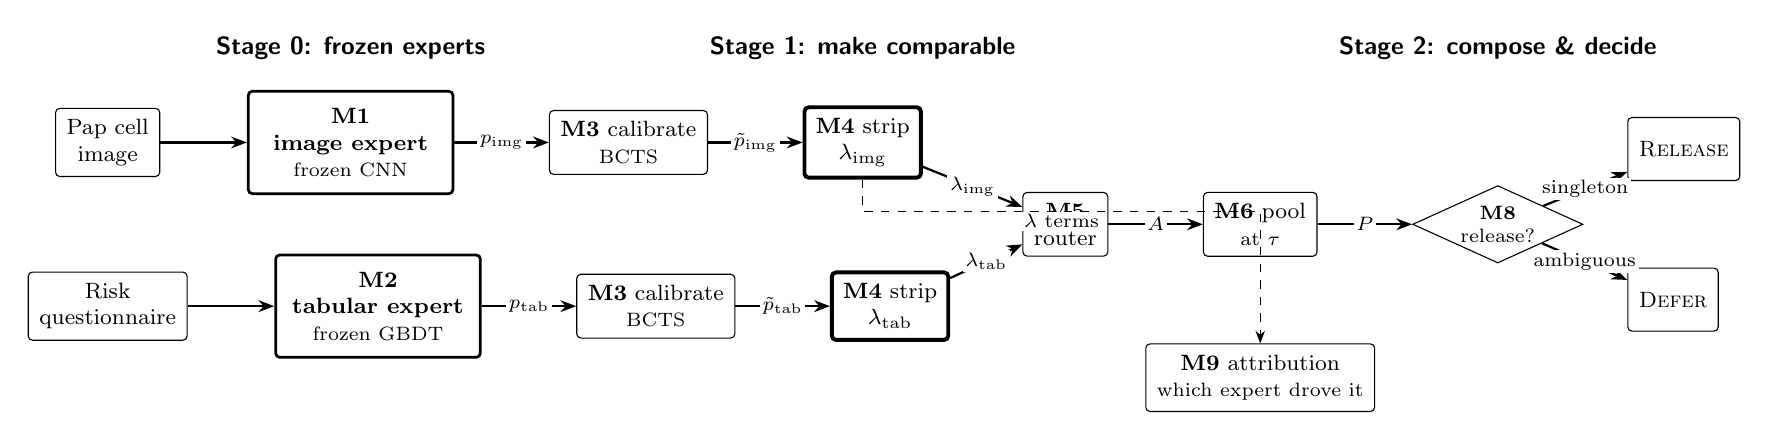
\begin{tikzpicture}[node distance=9mm and 13mm, newm/.style={box, line width=1.4pt}]
  \node[box] (xi) {Pap cell\\image};
  \node[bigbox, right=11mm of xi] (m1) {\textbf{M1}\\\textbf{image expert}\\\scriptsize frozen CNN};
  \node[box, below=12mm of xi] (xt) {Risk\\questionnaire};
  \node[bigbox, right=11mm of xt] (m2) {\textbf{M2}\\\textbf{tabular expert}\\\scriptsize frozen GBDT};
  \node[box, right=12mm of m1] (c1) {\textbf{M3} calibrate\\\scriptsize BCTS};
  \node[box, right=12mm of m2] (c2) {\textbf{M3} calibrate\\\scriptsize BCTS};
  \node[newm, right=12mm of c1] (s1) {\textbf{M4} strip\\$\lambda_{\mathrm{img}}$};
  \node[newm, right=12mm of c2] (s2) {\textbf{M4} strip\\$\lambda_{\mathrm{tab}}$};
  \node[box] (r) at ($(s1)!0.5!(s2)+(2.4,0)$) {\textbf{M5}\\router};
  \node[box, right=12mm of r] (p) {\textbf{M6} pool\\\scriptsize at $\tau$};
  \node[dec, right=12mm of p] (d) {\textbf{M8}\\release?};
  \node[box, above right=3mm and 11mm of d] (o1) {\textsc{Release}};
  \node[box, below right=3mm and 11mm of d] (o2) {\textsc{Defer}};
  \node[box, below=11mm of p] (m9) {\textbf{M9} attribution\\\scriptsize which expert drove it};
  \draw[fl](xi)--(m1); \draw[fl](xt)--(m2);
  \draw[fl](m1)-- node[lbl]{$p_{\mathrm{img}}$}(c1);
  \draw[fl](m2)-- node[lbl]{$p_{\mathrm{tab}}$}(c2);
  \draw[fl](c1)-- node[lbl]{$\tilde p_{\mathrm{img}}$}(s1);
  \draw[fl](c2)-- node[lbl]{$\tilde p_{\mathrm{tab}}$}(s2);
  \draw[fl](s1)-- node[lbl]{$\lambda_{\mathrm{img}}$}(r);
  \draw[fl](s2)-- node[lbl]{$\lambda_{\mathrm{tab}}$}(r);
  \draw[fl](r)-- node[lbl]{$A$}(p);
  \draw[fl](p)-- node[lbl]{$P$}(d);
  \draw[fl](d)-- node[lbl]{\scriptsize singleton}(o1);
  \draw[fl](d)-- node[lbl]{\scriptsize ambiguous}(o2);
  \draw[flthin,dashed](s1.south) -- ++(0,-4mm) -| node[lbl,pos=0.25,below]{\scriptsize $\lambda$ terms} (m9.north);
  \node[font=\bfseries\small] at (m1|-xi) [yshift=12mm] {\textsf{Stage 0: frozen experts}};
  \node[font=\bfseries\small] at (s1|-xi) [yshift=12mm] {\textsf{Stage 1: make comparable}};
  \node[font=\bfseries\small] at (d|-xi)  [yshift=12mm] {\textsf{Stage 2: compose \& decide}};
\end{tikzpicture}}
\caption{\textbf{End-to-end architecture.} Two experts trained on \emph{disjoint} cohorts are frozen (Stage 0); each posterior is calibrated and then has its own training prevalence divided out (Stage 1); the router admits any non-empty subset and the pool applies one declared prior $\tau$ once (Stage 2). \emph{Thick boxes are our contribution; thin boxes are deliberately borrowed.} Nothing after Stage 0 is trained on joint data, because no joint data exists.}
\Description{A left-to-right architecture with two parallel branches for image and questionnaire, each passing through a frozen expert, a calibration block and a prior-stripping block, then merging at a router and a pooling block, ending in a release-or-defer decision, with a dashed line to a modality-attribution block.}
\label{fig:arch}
\end{figure*}

\subsection{Module cards}

\paragraph{M1 --- Image expert (borrowed).}
\begin{itemize}
  \item \emph{Purpose.} Emit a cytomorphology posterior for one cell.
  \item \emph{Inputs / Outputs.} Cell image $x_{\mathrm{img}}$ / $p_{\mathrm{img}}$ and the training prevalence $\pi_{\mathrm{img}}$.
  \item \emph{Internal operations.} EfficientNet backbone~\cite{tan2019efficientnet}, optionally distilled for edge use~\cite{hinton2015distilling}; the five SIPaKMeD classes are collapsed to abnormal $=$ \{koilocytotic, dyskeratotic\}.
  \item \emph{Failure modes.} A $27$--$47$ point external collapse ($0.998\!\to\!0.73/0.59/0.53$); no patient IDs, so patient-wise splitting is impossible; koilocytosis marks \emph{productive} HPV and is a weak proxy for high-grade disease.
  \item \emph{Cost.} One forward pass.
  \item \emph{Novelty.} None claimed.
\end{itemize}

\paragraph{M2 --- Tabular expert (borrowed model, modified protocol).}
\begin{itemize}
  \item \emph{Purpose.} Emit a pre-test risk from the questionnaire.
  \item \emph{Inputs / Outputs.} $x_{\mathrm{tab}}$ / $p_{\mathrm{tab}}$, $\pi_{\mathrm{tab}}\approx0.064$.
  \item \emph{Internal operations.} Gradient-boosted trees~\cite{grinsztajn2022why} under a leakage-safe protocol: \texttt{Dx:*} dropped, resampling inside folds only, nested stratified CV, bootstrap CIs.
  \item \emph{Failure modes.} $14.6{:}1$ imbalance; $35$--$74$ positives per target; a single Venezuelan cohort with no external validation anywhere in that literature.
  \item \emph{Cost.} Seconds on CPU.
  \item \emph{Novelty.} The \emph{audit} is the contribution, not the model.
\end{itemize}

\paragraph{M3 --- Per-expert calibration (borrowed).}
\begin{itemize}
  \item \emph{Purpose.} Make each $p_k$ a genuine frequency \emph{before} any prior arithmetic.
  \item \emph{Internal operations.} Bias-corrected temperature scaling with maximum-likelihood label-shift estimation~\cite{alexandari2020maximum}, fitted on expert $k$'s own held-out fold; report ECE, Brier and a reliability diagram per expert.
  \item \emph{Why it is mandatory.} Prior correction presupposes a calibrated posterior---a condition ``not true of modern neural networks''~\cite{alexandari2020maximum}. Skip M3 and M4 is meaningless.
  \item \emph{Failure modes.} Few positives make the temperature high-variance; mitigated by cross-fitting.
  \item \emph{Novelty.} None claimed.
\end{itemize}

\paragraph{M4 --- Prior-stripping (\textbf{our contribution}).}
This is the module the proposal exists for, so it gets an analogy before the mechanism.

\begin{exbox}[Two thermometers, two rooms]
Two nurses each estimate ``is this patient feverish?''. Nurse A works in a fever clinic where $40\%$ of patients are feverish; Nurse B works in a general clinic where $6\%$ are. Both are well-calibrated \emph{in their own clinic}. If Nurse A says $70\%$ and Nurse B says $70\%$, they are \emph{not} saying the same thing: A's $70\%$ is barely above her baseline of $40\%$, while B's $70\%$ is a dramatic departure from her baseline of $6\%$. Averaging the two numbers silently treats the clinics' case mixes as if they were evidence about \emph{this} patient. The fix is to ask each nurse not ``how likely is fever?'' but ``\emph{how much did this patient's signs move you away from your own baseline?}''---and to add the baseline back exactly once, at the end, using the prevalence of the clinic where the system is actually deployed.
\end{exbox}

\begin{itemize}
  \item \emph{Purpose.} Remove each expert's own cohort prevalence, so that what is pooled is \emph{evidence} rather than evidence entangled with an accident of dataset construction.
  \item \emph{Inputs / Outputs.} $(\tilde p_k,\pi_k)$ / a prior-free log-likelihood-ratio $\lambda_k$.
  \item \emph{Internal operations.} Eq.~\eqref{eq:strip}; closed form, two logarithms.
  \item \emph{Failure modes.} $\pi_k$ must be \emph{known}: for a curated cohort it is a construction artefact, not a population rate. We therefore treat $\pi_k$ as a \emph{declared, audited} quantity and sweep it $\pm50\%$ (ablation A7). If $\tilde p_k$ is uncalibrated, $\lambda_k$ is not a likelihood ratio at all.
  \item \emph{Cost.} Microseconds; no training.
  \item \emph{Novelty.} \textbf{New.} Closest prior work sits on either side and never crosses: one-classifier prior correction~\cite{saerens2002adjusting,alexandari2020maximum,godau2023deployment} versus common-prior combination~\cite{kittler1998combining,genest1986combining,chen2022proben}.
\end{itemize}

\paragraph{M5 --- Availability router (borrowed).}
\begin{itemize}
  \item \emph{Purpose.} Accept any non-empty subset $A$.
  \item \emph{Internal operations.} An absent expert contributes $\lambda_k=0$, the additive identity---equivalently a vacuous opinion, the identity of Dempster's rule. \emph{No imputation}, which at zero overlap has nothing to impute from.
  \item \emph{Failure modes.} A lone weak expert must not auto-decide; it is routed to M8.
  \item \emph{Novelty.} None claimed --- this is ProbEn's marginalisation~\cite{chen2022proben}.
\end{itemize}

\paragraph{M6 --- Composition at a declared prevalence (borrowed rule).}
\begin{itemize}
  \item \emph{Purpose.} Produce the composed posterior with the prior counted exactly once.
  \item \emph{Internal operations.} Eq.~\eqref{eq:pool}; the robust sum rule of Eq.~\eqref{eq:sum} is evaluated alongside, since the tabular posterior is high-variance and the sum rule tolerates that better~\cite{kittler1998combining}.
  \item \emph{Failure modes.} The additive form \emph{is} naive Bayes and inherits its over-confidence (M7).
  \item \emph{Novelty.} None claimed. Only its \emph{inputs} are new.
\end{itemize}

\paragraph{M7 --- Dependence envelope (modified).}
\begin{itemize}
  \item \emph{Purpose.} Quantify the price of the assumption we cannot avoid.
  \item \emph{Internal operations.} Sweep $\rho\in[-1,1]$ in Eq.~\eqref{eq:env} over the \emph{real} marginals and report the range, not a point.
  \item \emph{Failure modes.} It is a model-based \emph{bound}, not a measurement, and is labelled as such on every figure.
  \item \emph{Novelty.} Modified: the envelope is standard; transporting the biostatistical penalty~\cite{grill2017comparison} into a pre-registered prediction about our own output is the new part.
\end{itemize}

\paragraph{M8 --- Per-path conformal abstention (borrowed, deliberately weakened).}
\begin{itemize}
  \item \emph{Purpose.} A reject option with a distribution-free guarantee.
  \item \emph{Internal operations.} Mondrian split conformal calibrated \emph{per expert on its own cohort}; a non-singleton prediction set triggers \textsc{Defer}.
  \item \emph{Honest scope.} We claim \emph{marginal, per-path} coverage only. Per-expert guarantees do not compose into a joint one, and the label-shift correction requires unlabeled target data that does not exist here~\cite{podkopaev2021distribution}.
  \item \emph{Novelty.} None claimed~\cite{angelopoulos2021gentle}.
\end{itemize}

\paragraph{M9 --- Modality attribution (modified).}
\begin{itemize}
  \item \emph{Purpose.} Report \emph{which} expert drove the call---free, because $\lambda_{\mathrm{img}}$ and $\lambda_{\mathrm{tab}}$ are on the same additive scale.
  \item \emph{Failure modes.} Explanation is not benefit: clinician-facing explanations did not mitigate the harm of a biased model in a randomised study of $457$ clinicians. We therefore claim no clinical benefit without a reader study.
  \item \emph{Novelty.} Modest; a read-out of M4.
\end{itemize}

\subsection{Mathematical formulation}

Calibrate first (M3), then strip (M4):
\begin{equation}
\lambda_k \;=\; \mathrm{logit}\big(\tilde p_k\big) \;-\; \mathrm{logit}\big(\pi_k\big).
\label{eq:strip}
\end{equation}

\emph{Reading Eq.~\eqref{eq:strip} term by term:} $\tilde p_k\in(0,1)$ is expert $k$'s calibrated probability that the case is abnormal; $\pi_k$ is the fraction of abnormal cases in the cohort that expert was \emph{trained} on. $\mathrm{logit}(x)=\log\frac{x}{1-x}$ converts a probability into log-odds, which turns the multiplication in Bayes' rule into addition. The subtraction is the whole idea: if the expert says exactly its own base rate ($\tilde p_k=\pi_k$) it has learned nothing about \emph{this} case and $\lambda_k=0$. The decisive quantity is the sign: $\lambda_k>0$ means ``this case looks \emph{more} abnormal than my average case'', $\lambda_k<0$ means less. Because $\lambda_k$ is a \emph{likelihood ratio}, it no longer depends on the training prevalence---which is exactly why it is transportable to a different cohort, and why $\tilde p_k$ is not.

The composition applies one declared prior:
\begin{equation}
\mathrm{logit}\,P\big(Y{=}1\mid \{x_k\}_{k\in A}\big) \;=\; \mathrm{logit}(\tau) \;+\; \sum_{k\in A} w_k \lambda_k .
\label{eq:pool}
\end{equation}

\emph{Reading Eq.~\eqref{eq:pool} term by term:} $\tau$ is the prevalence of the population where the system is actually deployed---a \emph{declared, auditable clinical input}, not something inherited from whichever dataset happened to be used. Each available expert adds its evidence $\lambda_k$, scaled by a reliability weight $w_k\in[0,1]$. An absent expert contributes nothing ($\lambda_k=0$), so $A=\{\mathrm{img}\}$ recovers the image-only path \emph{exactly}. With $w_k=1$ this is precisely ProbEn / naive Bayes~\cite{chen2022proben}; we claim no novelty in this line, only in what feeds it.

The robust alternative pools the anchored posteriors instead of the log-odds:
\begin{equation}
P_{\mathrm{sum}} \;=\; \frac{1}{|A|}\sum_{k\in A}\sigma\big(\mathrm{logit}(\tau)+\lambda_k\big).
\label{eq:sum}
\end{equation}

\emph{Reading Eq.~\eqref{eq:sum}:} each expert is first turned back into a probability \emph{at the deployment prevalence}, then averaged. Averaging cannot run away to $0$ or $1$ the way a sum of log-odds can, which is why Kittler et al.\ find the sum rule less sensitive to a single bad estimate~\cite{kittler1998combining}---relevant because our tabular expert is estimated from as few as $35$ positives.

Finally the envelope over the unknown dependence:
\begin{equation}
\mathrm{AUROC}_{\mathrm{fused}}(\rho) \;=\; \Phi\!\left(\frac{d_{\mathrm{img}}+d_{\mathrm{tab}}}{\sqrt{2}\,\sqrt{2+2\rho}}\right),
\quad d_k=\sqrt{2}\,\Phi^{-1}(\mathrm{AUROC}_k).
\label{eq:env}
\end{equation}

\emph{Reading Eq.~\eqref{eq:env} term by term:} $\Phi$ is the standard normal CDF. $d_k$ is the \emph{separation} of expert $k$---how far apart its scores sit for abnormal versus normal cases---recovered from its measured AUROC. $\rho$ is the correlation between the two experts' errors \emph{given} the true state: $\rho=0$ means they make independent mistakes (the optimistic case, where pooling helps most); $\rho=1$ means they make the \emph{same} mistakes, and the equation collapses to a single expert's AUROC---pooling adds nothing. Because both of our signals are driven by HPV, the honest operating region is $\rho>0$. At our measured marginals ($0.73$ external image, $0.65$ tabular) the gain is $+0.016$ at $\rho=0$ and $-0.030$ at $\rho=0.6$: composition stops paying almost immediately. The critical fact is that \emph{$\rho$ is non-identified at zero cohort overlap}---no estimator of it exists from our data---so we report the curve, not a number.

\subsection{Algorithms}

\begin{algorithm}[t]
\caption{CO-PRIOR fit (per expert, one cohort at a time)}
\label{alg:fit}
\footnotesize
\begin{algorithmic}[1]
\Require cohort $D_k$, frozen expert $f_k$, target coverage $1-\alpha$
\Ensure $(T_k,b_k)$, $\pi_k$, conformal thresholds $q_{k,c}$
\State split $D_k$ into fit / calibration folds (stratified)
\State $\pi_k \gets$ declared prevalence of $D_k$ \Comment{audited, not learned}
\State $(T_k,b_k) \gets \Call{BCTS}{f_k, \text{cal fold}}$ \Comment{M3}
\State $\tilde p \gets \sigma(z/T_k + b_k)$ on the cal fold
\State report $\mathrm{ECE}_k$, $\mathrm{Brier}_k$ \Comment{gate: M4 is invalid if uncalibrated}
\For{$c \in \{0,1\}$}
  \State $q_{k,c} \gets \mathrm{Quantile}_{1-\alpha}\big(\{1-\tilde p_{i,c} : y_i = c\}\big)$
\EndFor
\State \textbf{return} $(T_k,b_k), \pi_k, q_{k,\cdot}$
\end{algorithmic}
\end{algorithm}

\emph{Reading Algorithm~\ref{alg:fit}.} Every line touches \emph{one} cohort. Line 2 records the training prevalence as a declared quantity---we never estimate it from the other cohort, because the two cohorts share no patients. Line 3 fits the calibrator, and line 5 is a \emph{gate}, not a report: if the expert is not calibrated, the prior-stripping in Eq.~\eqref{eq:strip} does not yield a likelihood ratio and the rest of the pipeline is void. Lines 6--8 fit the conformal thresholds per class, on the same single cohort. Nothing here needs a paired sample---which is precisely why this proposal is testable.

\begin{algorithm}[t]
\caption{CO-PRIOR compose (inference, any subset)}
\label{alg:compose}
\footnotesize
\begin{algorithmic}[1]
\Require available $A\neq\emptyset$, raw $\{p_k\}_{k\in A}$, $\{(T_k,b_k),\pi_k,q_{k,\cdot}\}$, $\tau$, weights $w_k$
\Ensure composed $P$, decision, attribution
\State $z \gets \mathrm{logit}(\tau)$
\For{$k \in A$}
  \State $\tilde p_k \gets \sigma(\mathrm{logit}(p_k)/T_k + b_k)$ \Comment{M3}
  \State $\lambda_k \gets \mathrm{logit}(\tilde p_k) - \mathrm{logit}(\pi_k)$ \Comment{M4: strip}
  \State $z \gets z + w_k \lambda_k$ \Comment{M6: pool}
\EndFor
\State $P \gets \sigma(z)$
\State $C \gets \{c : 1-\tilde p_{k^\ast,c} \le q_{k^\ast,c}\}$ \Comment{M8, $k^\ast$ = strongest available}
\If{$|C| \neq 1$} \State \textbf{return} $P$, \textsc{Defer}, $\{\lambda_k\}$
\EndIf
\State \textbf{return} $P$, \textsc{Release}, $\{\lambda_k\}$
\end{algorithmic}
\end{algorithm}

\emph{Reading Algorithm~\ref{alg:compose}.} Line 1 seeds the accumulator with the \emph{deployment} prior, so it is counted once and only once. The loop runs over \emph{whatever arrived}: with only an image, only $\lambda_{\mathrm{img}}$ is added and the output is provably identical to the image-only path---graceful degradation is structural, not trained. Line 4 is the contribution. Line 8 asks the reject question against a per-expert conformal threshold, so the guarantee we quote is the one we can actually keep (marginal, per path). The returned $\{\lambda_k\}$ \emph{is} the explanation (M9): the two numbers are on one scale, so ``the image contributed $+2.1$, the questionnaire $-0.3$'' is a complete account of the decision.

\subsection{Decision policy}

\begin{figure}[t]\centering
\resizebox{0.95\columnwidth}{!}{%
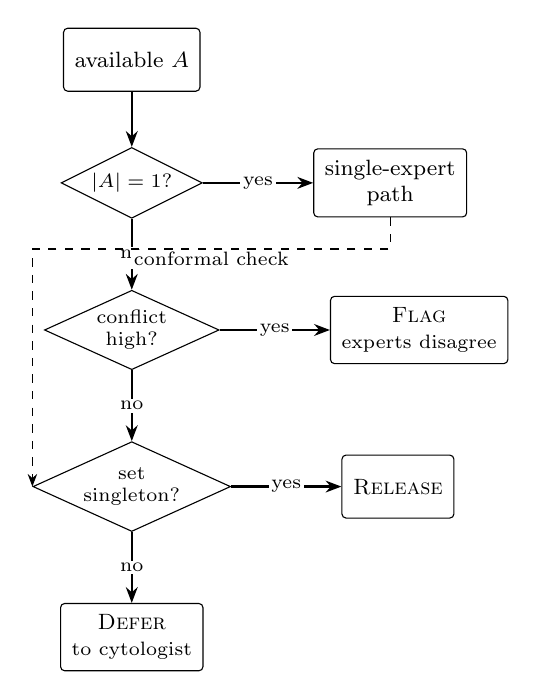
\begin{tikzpicture}[node distance=6mm and 12mm]
  \node[box] (in) {available $A$};
  \node[dec, below=7mm of in] (q1) {$|A|=1$?};
  \node[box, right=14mm of q1] (solo) {single-expert\\path};
  \node[dec, below=9mm of q1] (q2) {conflict\\high?};
  \node[box, right=14mm of q2] (flag) {\textsc{Flag}\\\scriptsize experts disagree};
  \node[dec, below=9mm of q2] (q3) {set\\singleton?};
  \node[box, right=14mm of q3] (rel) {\textsc{Release}};
  \node[box, below=9mm of q3] (def) {\textsc{Defer}\\\scriptsize to cytologist};
  \draw[fl](in)--(q1);
  \draw[fl](q1)-- node[lbl]{\scriptsize yes}(solo);
  \draw[fl](q1)-- node[lbl]{\scriptsize no}(q2);
  \draw[fl](q2)-- node[lbl]{\scriptsize yes}(flag);
  \draw[fl](q2)-- node[lbl]{\scriptsize no}(q3);
  \draw[fl](q3)-- node[lbl]{\scriptsize yes}(rel);
  \draw[fl](q3)-- node[lbl]{\scriptsize no}(def);
  \draw[flthin,dashed](solo.south) -- ++(0,-4mm) -| node[lbl,pos=0.25,below]{\scriptsize conformal check} (q3.west);
\end{tikzpicture}}
\caption{\textbf{Decision policy.} A lone weak expert never auto-releases; strong disagreement escalates rather than being averaged away.}
\Description{A flowchart from available modalities through checks on subset size, conflict and conformal set size to release, defer or flag.}
\label{fig:states}
\end{figure}

\begin{keybox}[Novelty boundary]
The \emph{prior-stripping precondition} is \textbf{our} contribution. The pooling rule, the router, the conformal reject option and the evidential conflict signal are deliberately \textbf{borrowed} and kept as separable modules---so the novelty stays cleanly the \emph{operator}, not the pipeline around it.
\end{keybox}

\subsection{Computational cost}

\begin{table}[t]
\caption{Cost. Everything after the frozen experts is closed-form.}
\label{tab:cost}
\footnotesize
\setlength{\tabcolsep}{4pt}
\begin{tabular}{@{}lll@{}}
\toprule
\textbf{Stage} & \textbf{Fit} & \textbf{Inference} \\
\midrule
M1 image expert & hours, 1 GPU & one forward pass \\
M2 tabular expert & seconds, CPU & $O(1)$ \\
M3 calibration & 2 scalars/expert & $O(1)$ \\
\textbf{M4--M6} & \textbf{none} & \textbf{$O(|A|)$, microseconds} \\
M8 conformal & one quantile/class & $O(1)$ \\
\bottomrule
\end{tabular}
\end{table}

The whole contribution runs on one $16$\,GB GPU because the only trained objects are two frozen experts and four scalars.

%% =====================================================================
\section{Novelty Statement}

We do \emph{not} claim the flexible any-modality architecture, the fusion rule, per-subset calibration, or modality dropout; those are~\cite{chen2022proben},~\cite{genest1986combining},~\cite{chlon2025aecf} and~\cite{gu2025modality} respectively, and we say so in the abstract. CO-PRIOR's differentiators, each checked against the primary sources: \textbf{(1)} the \emph{two-prior composition operator}---prior-stripping as a precondition of pooling, which the prior-correction literature (one classifier, one population~\cite{saerens2002adjusting,alexandari2020maximum,godau2023deployment}) and the combination literature (several classifiers, one common prior~\cite{kittler1998combining,genest1986combining,chen2022proben}) each leave to the other; \textbf{(2)} a \emph{leakage-audited} honest baseline for the field's most-used risk dataset, which no prior paper supplies; and \textbf{(3)} a \emph{pre-registered, directional} prediction of the over-confidence that a forced independence assumption must produce~\cite{grill2017comparison}, reported as an envelope because the dependence is non-identified. The scope is equally explicit: the both-modality path is \emph{unvalidatable} on public data, and we report that as a finding rather than papering over it with pseudo-pairing---a practice whose own dedicated critique we could locate~\cite{poh2006using} but not read.

%% =====================================================================
\section{Experimental Design}

\begin{table}[t]
\caption{Datasets and their roles.}
\label{tab:data}
\footnotesize
\setlength{\tabcolsep}{4pt}
\begin{tabular}{@{}lp{2.0cm}p{2.4cm}@{}}
\toprule
\textbf{Dataset} & \textbf{Role} & \textbf{What it tests} \\
\midrule
SIPaKMeD~\cite{plissiti2018sipakmed} & image train & in-distribution ceiling \\
Herlev & image external & transfer \\
HiCervix~\cite{cai2024hicervix} & image external & Bethesda-graded transfer \\
UCI 383~\cite{fernandes2017transfer} & tabular & honest ceiling, leakage \\
\emph{paired cohort} & \emph{none exists} & \emph{the impossibility} \\
\bottomrule
\end{tabular}
\end{table}

\paragraph{Model arsenal.}
Primary image expert: EfficientNet~\cite{tan2019efficientnet} (Apache-2.0, runs locally). Optional scale check: Smart-CCS~\cite{zhang2025smartccs}, the only cervical foundation model with strong external numbers \emph{and} a permissive licence (Apache-2.0, weights released). Tabular: gradient-boosted trees~\cite{grinsztajn2022why}. Note the licence inversion---general pathology foundation models are the \emph{most} restricted, with some forbidding deployed use entirely, while the cervical-specific models are the most permissive. \emph{Model-agnostic snapshot:} CO-PRIOR treats experts as black boxes emitting $(p_k,\pi_k)$, so any of these can be swapped without touching M3--M9.

\paragraph{Baselines.} Image-only (external, \emph{not} in-distribution); tabular-only (leakage-safe); \textbf{\texttt{max(image-only, tabular-only)} --- the key head-to-head}; raw pooling without stripping (isolates M4); ProbEn with a common assumed prior~\cite{chen2022proben}; the sum rule~\cite{kittler1998combining}; and a deliberate \emph{leaky reproduction} (SMOTE-before-split $+$ \texttt{Dx:*}) to show the published $0.98$--$1.00$ is an artefact.

\begin{table}[t]
\caption{Metrics. The headline is per-path net utility.}
\label{tab:metrics}
\footnotesize
\setlength{\tabcolsep}{4pt}
\begin{tabular}{@{}lp{4.6cm}@{}}
\toprule
\textbf{Metric} & \textbf{Definition / why} \\
\midrule
AUROC & discrimination; DeLong CI~\cite{delong1988comparing} \\
PR-AUC & mandatory at $4$--$12\%$ prevalence \\
ECE / Brier & calibration; the headline safety metric \\
signed cal.\ error & \emph{direction} of miscalibration (H-E) \\
coverage & conformal, per path, marginal \\
deferral rate & vs plausible cytologist workload \\
\bottomrule
\end{tabular}
\end{table}

\begin{keybox}[Pre-registered targets, not results]
Every number in Table~\ref{tab:accept} is a bar fixed \emph{before} the experiments are run. The falsifier row is included deliberately: we expect it may fire.
\end{keybox}

\begin{table*}[t]
\caption{Pre-registered acceptance criteria.}
\label{tab:accept}
\footnotesize
\setlength{\tabcolsep}{4pt}
\begin{tabular}{@{}llp{3.2cm}p{3.4cm}p{3.4cm}@{}}
\toprule
\textbf{Claim} & \textbf{Metric} & \textbf{Numeric bar (pre-registered)} & \textbf{Test} & \textbf{Result artifact} \\
\midrule
H-A honest ceiling & AUROC & upper 95\% CI $\le 0.75$ & BCa bootstrap, $10{,}000$ & CI table + forest plot \\
H-B leakage explains it & $\Delta$AUROC & honest $+$ leaks reconstructs published within $0.02$ & two-factor ablation & grouped bar $+$ 95\% CI \\
H-C stripping helps & $\Delta$ECE & $<0$, CI excludes $0$ & paired bootstrap & reliability diagrams \\
H-D confidence monotone & mean conf. & $0$ superset violations & bootstrap over patterns & confidence-vs-subset plot \\
\textbf{H-E falsifier} & AUROC & fused $\le$ \texttt{max(single)} at $\rho\ge0.3$ & DeLong~\cite{delong1988comparing} & envelope curve \\
\bottomrule
\end{tabular}
\end{table*}

\begin{table*}[t]
\caption{Experiment grid.}
\label{tab:expgrid}
\footnotesize
\setlength{\tabcolsep}{4pt}
\begin{tabular}{@{}llp{2.6cm}p{3.2cm}p{3.4cm}@{}}
\toprule
\textbf{ID} & \textbf{Experiment} & \textbf{Data} & \textbf{Comparison} & \textbf{Artifact} \\
\midrule
E1 & leakage-safe UCI re-benchmark & UCI & vs published $0.98$--$1.00$ & CI table \\
E2 & leakage decomposition & UCI & $\pm$\texttt{Dx:*} $\times$ $\pm$pre-split resample & grouped bar chart \\
E3 & per-expert calibration & UCI, SIPaKMeD & none/temp/BCTS/isotonic & reliability diagrams \\
E4 & \textbf{prior-stripping} & both & stripped vs raw vs post-hoc & ECE bar $+$ CI \\
E5 & dependence envelope & real marginals & fused vs \texttt{max(single)} & envelope curve \\
E6 & external transfer & Herlev, HiCervix & in-dist vs external & transfer matrix \\
E7 & any-subset degradation & both & $\{$img$\}$, $\{$tab$\}$, $\{$both$\}$ & confidence-vs-subset plot \\
E8 & abstention & both & risk--coverage & AURC curve \\
\bottomrule
\end{tabular}
\end{table*}

\begin{table*}[t]
\caption{Ablation grid. A6 is the ablation the proposal lives or dies by.}
\label{tab:abl}
\footnotesize
\setlength{\tabcolsep}{4pt}
\begin{tabular}{@{}llp{3.4cm}p{3.4cm}p{2.6cm}@{}}
\toprule
\textbf{ID} & \textbf{Removed / changed} & \textbf{Claim it isolates} & \textbf{Expected effect (grounded)} & \textbf{Artifact} \\
\midrule
A3 & \texttt{Dx:*} back in & target leakage (G5) & $0.592 \!\to\! 0.998$ (measured) & bar chart \\
A4 & resample before split & resampling leakage & reproduces $\approx0.98$--$1.00$~\cite{roy2025interpretable} & bar chart \\
A5 & target choice & estimand & Citology $0.488$, Hinselmann $0.450$ are $\le$ chance & CI table \\
\textbf{A6} & \textbf{stripping OFF} & \textbf{M4 --- the contribution} & \textbf{if $\Delta$ECE $\approx0$ the claim dies} & ECE bar $+$ CI \\
A7 & $\pi_k$ mis-specified $\pm50\%$ & robustness of M4 & degradation grows with error & line plot \\
A8 & $\tau$ sweep & declared prior & the fused number is meaningless without $\tau$ & line plot \\
A9 & pool rule & product vs sum & sum more robust at $35$ positives~\cite{kittler1998combining} & bar chart \\
A11 & calibration off & M3 is a precondition & $\lambda$ ceases to be an LLR & reliability diagram \\
A14 & evidential $u$ as weight & G6 & degrades: $u$ is relative, not absolute & bar chart \\
\bottomrule
\end{tabular}
\end{table*}

\paragraph{Statistical analysis.}
\begin{itemize}
  \item AUROC differences: DeLong for correlated ROCs on the same cases~\cite{delong1988comparing}; BCa bootstrap ($10{,}000$ resamples) elsewhere.
  \item ECE differences: paired bootstrap with BCa intervals.
  \item Multiplicity: the primary family is \{H-C, H-E\}; Holm--Bonferroni. Everything else is secondary and labelled so.
  \item Variance: $\ge5$ repeats of stratified CV with recorded seeds; report mean $\pm$ SD \emph{and} the pooled-OOF bootstrap CI.
  \item \emph{Power, stated honestly:} with $55$ biopsy positives the AUROC CI half-width is $\approx0.07$. We therefore pre-declare that tabular-arm differences below $0.05$ AUROC are \textbf{not resolvable} and will not be claimed.
\end{itemize}

\paragraph{Result artifacts.} Each analysis has one required output: reliability diagrams (E3, E4, A11); grouped bar $+$ 95\% CI (E2, A3, A4); the dependence envelope curve (E5, H-E); a transfer matrix heatmap (E6); a confidence-vs-availability plot (E7, H-D); a risk--coverage (AURC) curve (E8); and a CI/forest table (E1, A5).

%% =====================================================================
\section{Threats to Validity and Limitations}

\begin{itemize}
  \item \emph{Construct (severe).} $p_{\mathrm{img}}$ and $p_{\mathrm{tab}}$ measure different things on different units (Fig.~\ref{fig:2x2}). \emph{Mitigation:} latent-indicator framing~\cite{rutjes2007evaluation}; every composed number is reported conditional on that model.
  \item \emph{Internal.} $\pi_k$ for a curated cohort is a construction artefact. \emph{Mitigation:} declared and audited, swept $\pm50\%$ (A7).
  \item \emph{External (fatal to the headline path).} No paired cohort exists, so joint discrimination and calibration are unmeasurable. \emph{Mitigation:} none possible; we report it as the finding and cost a prospective pilot instead.
  \item \emph{Statistical.} $35$--$74$ positives per UCI target; differences $<0.05$ AUROC are not resolvable and are not claimed.
  \item \emph{Clinical.} A weak questionnaire must never lower a positive cytology call. \emph{Mitigation:} the questionnaire may only raise suspicion or trigger deferral.
  \item \emph{Novelty risk.} If A6 shows prior-stripping is numerically equivalent to a single post-hoc correction, the operator is a re-parameterisation and the contribution collapses---in which case this work is demoted to a \emph{diagnostic study}: the leakage audit plus the impossibility result, reported as such.
\end{itemize}

%% =====================================================================
\section{Conclusion}

A flexible cervical screener that accepts an image, a questionnaire, or both is blocked not by architecture but by data: the two public signals share no patients, no labels, and no unit of analysis. We proposed CO-PRIOR, whose single claim is small and testable---strip each expert's own training prevalence out before pooling, and apply one declared deployment prior afterwards---because that is the one operation the prior-correction and classifier-combination literatures each leave to the other, and because it can be validated one cohort at a time, which is the only validation this data permits. Everything else is deliberately borrowed and named. The leakage-audited baseline ($0.656$ against a published $0.98$--$1.00$) and the pre-registered falsifier are what make the proposal falsifiable rather than merely plausible; if fusion does not beat the better single expert, we will say so.

\bibliographystyle{ACM-Reference-Format}
\bibliography{refs}

\end{document}
